\subsubsubsection{Kiến trúc chi tiết của hệ thống}

Hệ thống được thiết kế theo mô hình \textbf{Layered Architecture}. Luồng xử lý chính của hệ thống tuân theo quy tắc phụ thuộc chặt chẽ: một lớp ở trên chỉ có thể giao tiếp với lớp ngay bên dưới nó. Dữ liệu yêu cầu sẽ đi từ lớp trên cùng (Presentation Layer) xuống các lớp dưới để xử lý và truy xuất dữ liệu, sau đó dữ liệu phản hồi sẽ được trả ngược lên trên.
\begin{landscape}
\begin{figure}[htp]
    \centering
    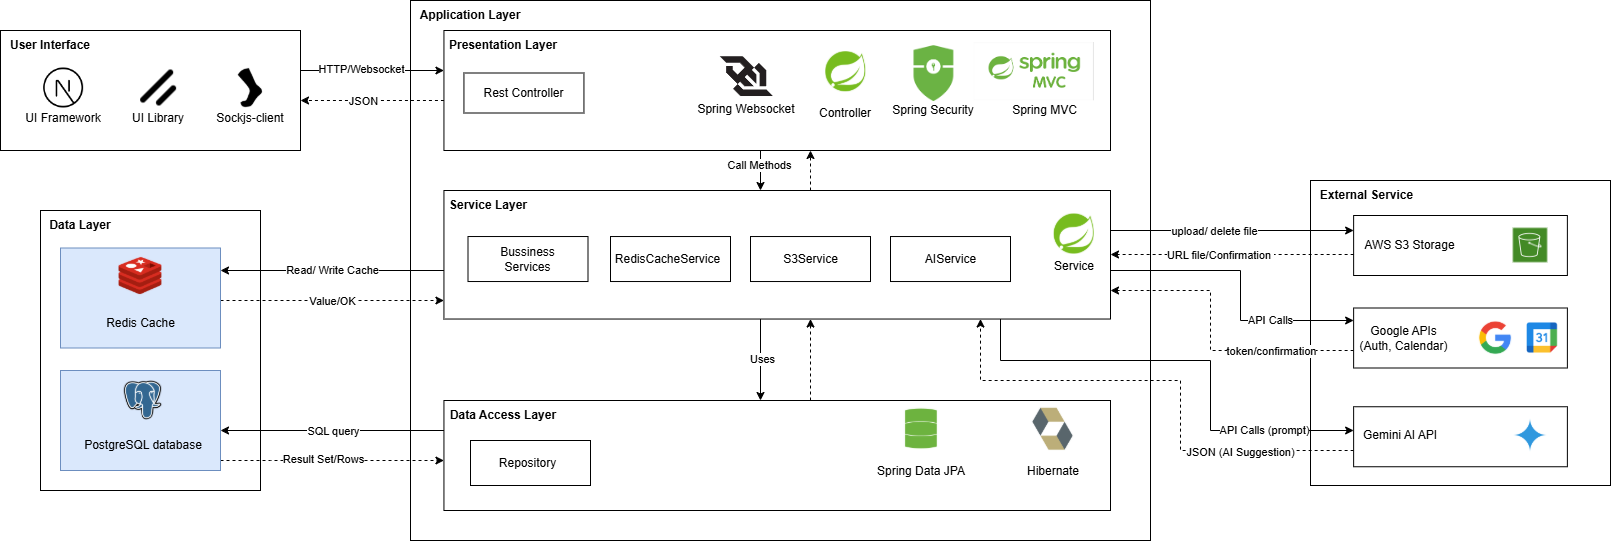
\includegraphics[width=1.6\textwidth]{Images/7. System Design/system_architecture.png}
    \caption{Kiến trúc hệ thống}
    \label{fig:system_architecture} 
\end{figure}  
\end{landscape}
Các tầng trong kiến trúc hệ thống:
\begin{itemize}
    \item \textbf{User interface}: Đây là tầng trên cùng của kiến trúc, chịu trách nhiệm tương tác trực tiếp với người dùng cuối. 
    \item \textbf{Application Layer}: Đây là lõi của hệ thống, chứa toàn bộ logic nghiệp vụ và điều phối hoạt động giữa các tầng khác. Tầng này được chia nhỏ thành 3 lớp con:
    \begin{itemize}
        \item \textbf{Presentation layer}: Là cửa ngõ giao tiếp của backend, tiếp nhận các yêu cầu từ Tầng Giao diện người dùng. Lớp này xác thực, phân quyền, và kiểm tra tính hợp lệ của dữ liệu đầu vào trước khi chuyển đến Service layer. Lớp này hiển thị tài nguyên của hệ thống ra bên ngoài dưới dạng các API.
        \item \textbf{Service layer}: Thực thi toàn bộ logic nghiệp vụ của ứng dụng. Đây là nơi các quy trình phức tạp được xử lý (xử lý yêu cầu tạo lộ trình bằng AI, quản lý đánh giá của cộng đồng, xử lý thông báo, và tích hợp với các dịch vụ bên ngoài, …). Lớp này điều phối các hoạt động giữa tầng \textbf{Data access layer} và các dịch vụ khác.
        \item \textbf{Data access layer}: Cung cấp một lớp trừu tượng để giao tiếp với Data Layer. Nó chịu trách nhiệm thực hiện các thao tác CRUD trên cơ sở dữ liệu và che giấu sự phức tạp của các câu lệnh truy vấn SQL.
    \end{itemize}
    \item \textbf{Data layer}: Tầng này chịu trách nhiệm lưu trữ và quản lý toàn bộ dữ liệu của hệ thống một cách bền vững.
    \item \textbf{External Service}: Tầng này bao gồm các dịch vụ của bên thứ ba được tích hợp để mở rộng và nâng cao chức năng cho hệ thống.
\end{itemize}